\documentclass[12pt]{article}
\usepackage{fancyhdr}
\usepackage{nopageno}
\usepackage{lastpage}
\setlength{\headheight}{15.2pt}
\renewcommand{\headrulewidth}{0pt}
%\pagestyle{fancy}
\usepackage{graphicx}
\usepackage{geometry} % see geometry.pdf on how to lay out the page. There's lots.
\usepackage[utf8]{inputenc}
\usepackage{gb4e}
\usepackage[T1]{fontenc}
\usepackage{ tipa }
\usepackage{qtree}
\usepackage{amssymb}
\usepackage{epstopdf}
\usepackage{qtree}
\usepackage{tree-dvips}
\usepackage{natbib}
\usepackage{hyperref}
\usepackage{soul}


\geometry{letterpaper} % or letter or a5paper or ... etc
\bibpunct{(}{)}{;}{a}{}{,}
\renewcommand{\theenumi}{\alph{enumi}}
%\renewcommand{\thesection}{}

% \geometry{landscape} % rotated page geometry

% See the ``Article customise'' template for come common customisations



%%% BEGIN DOCUMENT
\begin{document}

%\maketitle
\noindent Is Uniformity Important in Uniform Information Density?\\
Is smoothness at issue in the smooth signal redundancy hypothesis?\\
\noindent Joel C. Wallenberg\\

\section{Introduction}

\nocite{shannon1948reprint}
In 1929, working on the thermodynamics problem known as Maxwell's Demon, Leo Szilard published an article proposing that an observer's uncertainty about the outcome of an event was a type of entropy, and could be measured in binary digits (``bits''). This fundamental insight was mostly overlooked until \citet{shannon1948} developed a full theory of how to quantify information. He defined the amount of information a sender could theoretically communicate as the amount of uncertainty a potential receiver has, regarding whatever the sender intends to describe. Shannon went on to demonstrate that communication only takes place when some signal removes uncertainty in the real or electrical mind of the receiver, including the binary electrical circuits that would begin the digital computer revolution. The birth of computer science led to the birth of formal (mathematical) linguistics, and early computational engineers such as John R. Pierce expected Shannon's information theory to be combined with formal linguistics \citet{pierce1980}. Sadly, these fields showed little sign of uniting until very recently. The hypothesis that speakers subtly manipulate linguistic structure so that their utterances are more resistant to ``noise'', in the information theoretic sense: any interference to a signal, including acoustic noise, interruption, memory failure, etc. Importantly, speakers do this naturally at different levels of granularity (e.g. syntax, words, phonemes). I believe this indicates a deep cognitive ability in humans for efficient within-brain communication, which exposes itself in the unconscious patterns of language.

For any event or situation with a number of possible outcomes, \citet{shannon1948} defined the ``information content'' in bits of each observable outcome as $log_2 \frac{1}{p_i}$, where $p$ is the probability of that observation. The lower the probability of an observation, the higher the information content, which follows the intuition that more surprising observations are more informative. For a hearer listening to a sentence, more rare linguistic items (e.g. ``concertina'') tend to reduce the hearer's overall uncertainty about the speaker's meaning more than very common linguistic items (e.g. ``the''). If some disturbance obscures ``concertina'', more information is therefore lost than if noise obscures ``the''.


\citet{shannon1948} wrote the following formula for the overall amount of information in some event with \textsl{n} discrete outcomes, if the possible outcomes have probabilities p_1...p_n. It gives the amount of information in ``bits'', which is also the number of binary circuits in a digital computer it would take to encode which outcome actually happened.

\begin{center}
	$$\sum_{1}^{n} p_i log_2 \frac{1}{p_i}$$
\end{center}

\noindent The $log_2 \frac{1}{p_i}$ part is the ``information content'' each possible outcome, and is the part we will concern ourselves with for this proposal. The lower the probability of an outcome, the higher the information content, which follows the intuition that more surprising events are more informative. For an interlocutor listening to a sentence that someone is saying, the information content of each linguistic unit coming from the speaker is its probability, and more rare linguistic items (e.g. ``concertina'') tend to reduce the hearer's overall uncertainty about the speaker's message more than very common linguistic items (e.g. ``the''). If some disturbance obscures ``concertina'', more information is therefore lost than if noise obscures ``the''.

%editing below this point

define: \textsl{signal} \textsl{channel}; \textsl{source}, or \textsl{message}, the outcome of some event that the sender wants the receiver to perceive (e.g. speaker's intended meaning or social function of an utterance); \textsl{noise}

Importantly, information theory recognizes that no message is truly encapsulated in a signal, like a letter in a bottle; rather, the message is re-constituted by the receiver, and the receiver does so by approaching the signal with some prior idea about the space of possible messages they might receive. They then use the signal to decide how probable the different possible messages in their set of priors, eventually zeroing in on the intended message, of getting as close as possible if signalling is imperfect (i.e. as it will be if there is noise in the channel, making the \textsl{mutual information} between the signal and message less than the total information of the message). Thus, information content isn't exactly a measure of how much of a message is encapsulated in the signal, but rather a measure of how much help that particular signal will be to the receiver in ``reconstructing the message from the signal'' in the words of \citet{shannon1948}. This reasoning will become particularly important in section \ref{moreity}.

In the last decade or so, there has been a renewal of interest in information theory as an explanatory mechanism for patterns of natural language use on the part of experimental, theoretical, and computational linguists. Much of the recent attention has focused on some version of the hypothesis that, given the choice, speakers prefer smoother or more uniform information distributions in the sentences they produce, rather than ones with large troughs and peaks in their information content. The studies testing this hypothesis, however, either do not test it directly, or they contain the following confound: the more uniform linguistic options they consider are also always longer than the less uniform option. This leads us to ask: is the information uniformity of utterances actually important in itself, or just their length? We suggest that once information uniformity and message-length are dissociated, uniformity turns out to still be important, but because it prevents catastrophic losses of entire utterances (or propositions) such that they are not recoverable; uniformity does not guard against information loss in general. 
 

\section{Research Context}
\label{context}

\subsection{Smooth Signal Redundancy Hypothesis and Uniform Information Density}

This renewed interest in information theory and language begins with \citet{aylettturk2004}'s ``Smooth Signal Redundancy Hypothesis'' (SSH), an application of \citet{shannon1948}'s Noisy Channel Coding Theorem to phonological production. Shannon's theorem has the consequence signals are less susceptible to noise disturbances if they are longer and/or more redundant in the way they encode information. \citet{aylettturk2004} claim that speakers prefer to spread information across their utterances as uniformly as possible, which prevents information-dense patches of speech where random noise could potentially destroy large amounts of information at once. Their corpus study showed that speakers manipulate durations at the phoneme, syllable, and word level, so that phonological units that are more information-dense (i.e. lower probability) are produced more slowly.

Speakers did this naturally and unconsciously, adjusting the durations of phonological constituents such that information distributed across utterance time as smoothly as possible. Speakers therefore seem to be adopting a strategy that follows naturally from Shannon's original Coding Theorem: codes that require longer signals distribute information at a lower rate per unit of code, which means they will lose information to noise at a lower rate than shorter-signal codes, given the same amount of noise per unit of time. But note that longer-signal codes distribute information more uniformly \textbf{by virtue of their length} (and codes with built-in redundancy are a special case), so speakers' preference for information uniformity in \citet{aylettturk2004} could just be a preference for longer signals.

\citet{levyjaeger2007} and \citet{jaeger2010} provide evidence that \citet{aylettturk2004}'s SSRH also applies to syntactic units, and renamed it ``Uniform Information Density''. However, here too, smoothness/uniformity is confounded with utterance length.  They show that, in relative clauses such as the one in \ref{rel}, the information content of the following word and phrase phrase affected speakers' choice to pronounce or omit the complementizer \textsl{that} (\citealt{jaeger2010} studied the same variable in complement clauses):

\begin{exe}
\ex \label{rel} How big is the family $[$(that) you cook for$]$?
\end{exe}

\noindent From the point of view of a hearer, the complementizer signals the beginning of the relative clause, but no other information.\footnote{\textsl{that} signals no other information, aside from the \textsl{that}-trace effect; taking that into account, \textsl{that} also decreases the probability of a following subject extraction for a hearer.} When \textsl{that} is omitted, the beginning of the relative clause is signalled by the first word in the clause (i.e. \textsl{you} in \ref{rel}), which information it bundles together with the information it carries by virtue of its lexical identity. They showed that speakers are less likely to omit \textsl{that} if the following word and/or following phrase (i.e. the subject of the relative and the first word of the subject) is high in information content, demonstrating an increasing preference for spreading the information content of the beginning of the relative across more words as that information content increases.

Levy and Jaeger interpret this result as a speaker bias towards producing more uniform information distributions. But again, the more uniform, more dispersed, distribution of information in sentences with an overt \textsl{that} results from the addition of a morpheme to the string. Just as \citet{aylettturk2004} were comparing phonological units of longer and shorter durations, Levy and Jaeger are comparing sentences with more or fewer words. And similarly, the information uniformity/smoothness they observe is a product of signal length, and speakers prefer longer signals in situations where information would otherwise become bunched up in part of a sentence. They have not tested whether speakers prefer more informationally uniform sentences when their options are the same length, and therefore whether uniformity itself is at issue.


\subsection{Building on SSRH and UID}

Following on from these seminal articles, there's been a fair bit of recent research that has mentioned the SSRH/UID hypotheses, but nearly all of them fail to consider the impact of information uniformity, i.e. the actual shape of the information distribution in utterances, independently of the length of the signal. \citet{frankjaeger2008}, for instance, make the same argument as the studies above, but with data from contractions (e.g. \textsl{I'm} for \textsl{I am}). Again, the two variants considered for their relative information uniformity differ in length. It's worth noting that, like \citet{levyjaeger2007} and \citet{jaeger2010}, this study calculates conditional entropy of a word given two preceding words and one following. This means that they do not attempt to characterize the shape of the information distribution of a whole utterance, but rather consider the density of the very local surroundings of the relevant linguistic variable, and rely more on preceding context than following. \citet{shannon1948}'s noisy channel coding theorem, however, applies to properties of whole signals, and so we should consider information distributions across whole utterances if possible, at least as far as working memory allows. The gap in the current literature, then, has two aspects: (a) considering the effect of uniformity, independent of length, and (b) considering the shape of distributions across whole utterances. The additional articles reviewed below do not constitute an exhaustive review, but we believe are a representative sample of recent studies.

The recent computational literature shows a number of relevant results, but do not quite show that speakers manipulate the information distributions of utterances to maximize uniformity. \citet{xureitter2016, xureitter2018} consider whether entropy peaks and troughs overlap between interlocutors in two-person discourses. They show that speakers tend to overlap in their average per-word entropy over segments of the discourse, but they do not assess the uniformity of entropy distributions over sentences or discourse turns, either between or within individual speakers. They also calculate per-word conditional entropy based on the two preceding words, but do not consider any other within-utterance linguistic context. \citet{doylefrank2015}, building on \citet{genzelcharniak2002}, show that the average rate of information across a discourse increases in absolute terms, but stays constant controlling for surrounding context. Studies like these show that there is broadly a steady average rate of per-word information transmission across a discourse, which can nevertheless change in response to major discourse shifts. They do not characterize the shape of information distributions across utterances or discourses, or show that more uniform shapes are preferred over other possible shapes given the same information to be communicated.

\citet{coupeetal2019} is a recent and rare attempt to estimate the optimal information rate in human language (in bits per second), which makes it an important step in eventually estimating the \textsl{channel capacity} of human language; the channel capacity is the highest rate at which a given channel can transmit information with an arbitrarily low error rate \citet{shannon1948}. As important as this step is, their study only considers a bias towards information uniformity to the extent that this reflects speakers' unwillingness to transmit information at too high a rate. Once again, uniformity per se is not really at issue here independent of length of the signal; a series of signal can be kept under channel capacity with appropriate choice of signal length and density of information per unit of code, regardless of the shape of the information distribution in the signal. \citet{coupeetal2019} do, however, make a strong case for a particular average rate of information transmission as a linguistic universal, and indirectly for a cognitive, pre-linguistic origin of the information manipulation we see in language, since speakers of different languages show remarkably little difference in information rate (bits/s).


There are just a couple notable exceptions in the recent literature, studies that are concerned with the shape of information distributions across utterances, and this more or less uniform shape independent of utterance length. \citet{temperleygildea2015} do look at information density independent of length of utterance, though they do not seem to realize this is a departure from much of the earlier ``UID'' literature. Their study considers information density in coordinated DP/NPs, and in particular, the combination of syntactic and lexical information in second conjuncts. They show that in second conjuncts, an increase in syntactic information content is, to some extent, counterbalanced by a decrease in lexical information (and vice-versa). This is certainly a relevant result for information uniformity, and shows that speakers avoid particularly dense bundles of information resulting from the combination of high syntactic and lexical information. The do not show, however, whether these bundles are particularly dense given the rest of the information in the utterance; informational uniformity of the utterance, taken seriously, does not mean there are no dense phrases in an absolute sense, but rather that phrases across the utterance are of similar density on average.  The study implicitly considers the context of the preceding conjunct, based on an argument that syntactically parallel second conjuncts are lower in information than first conjuncts, but this is still a very local syntactic relationship, and a left-to-right one; the next step is to consider information uniformity across whole utterances and in both directions. 

The other notable exception in the literature of a study that comes close to this goal is \citet{mauritsetal2010}. A direct test of speaker preference for informational uniformity would contrast alternative expressions of the same length, but with differently-shaped distributions of information content. \citet{mauritsetal2010} do compare word order variants of the same length, but do not seem to realize they've done something different from the previous SSH/UID literature, and do not propose a mathematical method for comparing information uniformity that is as general as the one we propose in section \ref{disentangle}.\footnote{They actually just barely stop short of doing this: they do have a way of comparing information uniformity between the set of 3-word sentences and 3-word experimental stimuli they consider, and they state what could be fleshed out to an even more general method: amount of linearity to the series of left-to-right conditional word entropies. We note, however, that this is more difficult to operationalize than the method we propose: first, because it involves model estimation and comparing derived goodness of fit statistics; secondly, because it can only consider information distributions from left-to-right but not right-to-left, and the noisy coding theorem should apply in both directions; and thirdly, it will be difficult to compare highly non-linear distributions to each other.} 

To give an example of the kind of comparison that would test uniformity directly, the sentences in (\ref{top}) and (\ref{relex}) below differ only in word order, not in length, and speakers have a free choice between them in some contexts.\footnote{It is, of course, well known that the object-fronting variant in (\ref{top}a) is only available in certain discourse contexts. But in those contexts, speakers still have a choice between that variant and the \textsl{in situ} (\ref{top}b) variant \citep{prince1998, prince1999}. There are many such examples of syntactic optionality within a particular context.} 

\begin{exe}
	\ex \label{top} \begin{xlist} \ex She likes carrots, not beets.
		\ex Carrots she likes, not beets.
		\end{xlist}
	\ex \label{relex} \begin{xlist}
		\ex I see a woman who's very important in that room.
		\ex I see a woman in that room who's very important.
	\end{xlist}
\end{exe}

\noindent To test whether information uniformity, per se, is preferred by speakers, we should look at variant pairs like those above in contexts where one or the other variant results in a more uniform, smoother information distribution across the entire sentence. This would dissociate the effect of uniformity from the effect of smoothing the distribution by adding length to the signal, or adding redundancy to the signal by adding length (both of which are equivalent from an information theoretic point of view, and covered by Shannon's original Noisy Coding Theorem). To do this, of course, we need a way of measuring the uniformity/smoothness or lack thereof (which we might call ``clumpiness'') of an information distribution for an entire utterance. We then need to answer the question: is uniformity, in and of itself, adaptive for linguistic communication in some way?



\section{Disentangling uniformity and redundancy}
\label{disentangle}

We've approached this problem by developing a novel and simple test statistic for assessing information uniformity across a whole utterance (i.e. in a string of words, morphemes, or phrases), and an algorithm that allows us to normalize our test statistic for comparison between utterances. The combination means that we can readily compare the uniformity or clumpiness of one whole utterance to another independently of the length of that utterance or how much information is being transmitted by the utterance overall. Thus, we have answered our two critiques of the literature in section \ref{context}: we can characterise the overall shape of the information distribution of an utterance, and we can do so independently of the length of an utterance. This puts us in a good position to answer what, if anything, uniformity is good for. In the simulation we present below, we answer that uniformity is indeed important for maximizing the information transmitted in a context of random noise, particularly when the noise is of an analog quality (e.g. acoustic noise) and the coding scheme is categorical (as most aspects of language are). Interestingly, though, uniformity does not result in less information lost overall under these conditions; rather, it results in fewer entire utterances being destroyed.

The test statistic, the ``Deviation of the Rolling Mean'' (DORM), provides a concise and easily interpretable summary of how uniform or clumpy a particular utterance is, while the normalization procedure, ``Uniform Information Density Optimization'' (UIDO), allows us to control for the length of an utterance and the overall amount of information the utterance is intended to transmit. Given a sentence and a list of information content measures for its word based on word probabilities (or morphemes or phrases -- the method is fully general), we take the arithmetic mean of every adjacent, overlapping pair of information content numbers, i.e. a rolling mean. We then compute the standard deviation of the resulting list of means and arrive at a single number, the DORM, which concisely measures the overall smoothness of the sentence's information distribution. A high DORM means that overlapping sequences of adjacent words are often very different to each other in information content, i.e. there are clumps of information, peaks and troughs that mean the sentence is less uniform. A low DORM indicates a more uniform string. Finally, we add a small penalty proportional to the number of possible unique permutations of the string, which helps prevent artificially low DORMs arising by chance in very short strings or repetitious strings (see ANONYMOUS, \textsl{Under Review}, and Supplementary Files for details).

The DORM's companion normalization procedure algorithm is ``Uniform Information Density Optimisation'' (UIDO). For any string of information content values, UIDO systematically reorders them, seeking to minimize the DORM for the whole string. UIDO halts once no additional permutation yields a lower DORM (for more details, see a full description in ANONYMOUS, \textsl{Under Review}). We thus arrive at a theoretical optimally uniform order for any string, and subtracting the DORM for the UIDO order from the string's actual DORM is a normalized measure that can be compared between utterances; each sentence gets a value for how uniform it is compared to how uniform it theoretically could be, given the words in the sentence (or morphemes, phrases, etc.).

The simulation below uses UIDO to show that optimally uniform sequences are more resistant to noise than other sequences, controlling for length of the sequence. We generated 10,000 hypothetical utterances, each consisting of 10 randomly generated probabilities to represent word frequencies, and then we converted these to Shannon-information content in bits by $$log_2 \frac{1}{p}$$. We created three versions of each ``sentence'' of information content values: its original, random order; a maximally asymmetric order of greatest-to-smallest values; and finally, a maximally uniform order that has been optimized for low DORM with the UIDO algorithm.

To simulate noise, we randomly identified a sequence of three numbers from each hypothetical sentence version, as if noise had obscured three words in a row. This three-item noise-obscured sequence began at the same position in the string in each of the three versions of each of the 10,000 trials of the simulation. In other words, for a given trial, if we suppose noise knocked out the first three words, it knocks out the first three words in the randomized version of that hypothetical sentence, the first three words in the asymmetric greatest-to-least version, and the first three in the UIDO version. This kind of noise was chosen because it is a realistic kind of noise for linguistic situations: typical types of noise in conversation, e.g. interfering acoustic noise, momentary lack of attention, short-term memory failure, can all be thought of as continuous types of noise that often span over multiple linguistic units, e.g. multiple words or morphemes. There are also types of categorical noise that will affect only single linguistic units, such as some speech errors, failure of word/morpheme recognition, word/morpheme retrieval failure, some mishearings, but we would expect language to be optmized to resist both types of noise simultaneously (not the categorical type alone), if language is optimized at all.

In the 10,000 trials of the simulation, the UIDO-optimized order did not do any better than the asymmetric order in preserving the most number of bits overall, but the UIDO order did result in the fewest hypothetical utterances disturbed by extremely large losses of information, which we'll call ``catastrophic communication failures'' (Figure \ref{sim}). For each trial, i.e. each set of three versions of the same set of information content values, we looked out how many bits of information were obscured by noise in each version, and what proportion of the total information in that hypothetical sentence was destroyed.  In addition to the proportion of total bits destroyed, we also considered whether some version of that sentence suffered a catastrophic communication failure, which we defined as a loss of more than half the information in the hypothetical sentence. 

\begin{figure}
	\begin{center}
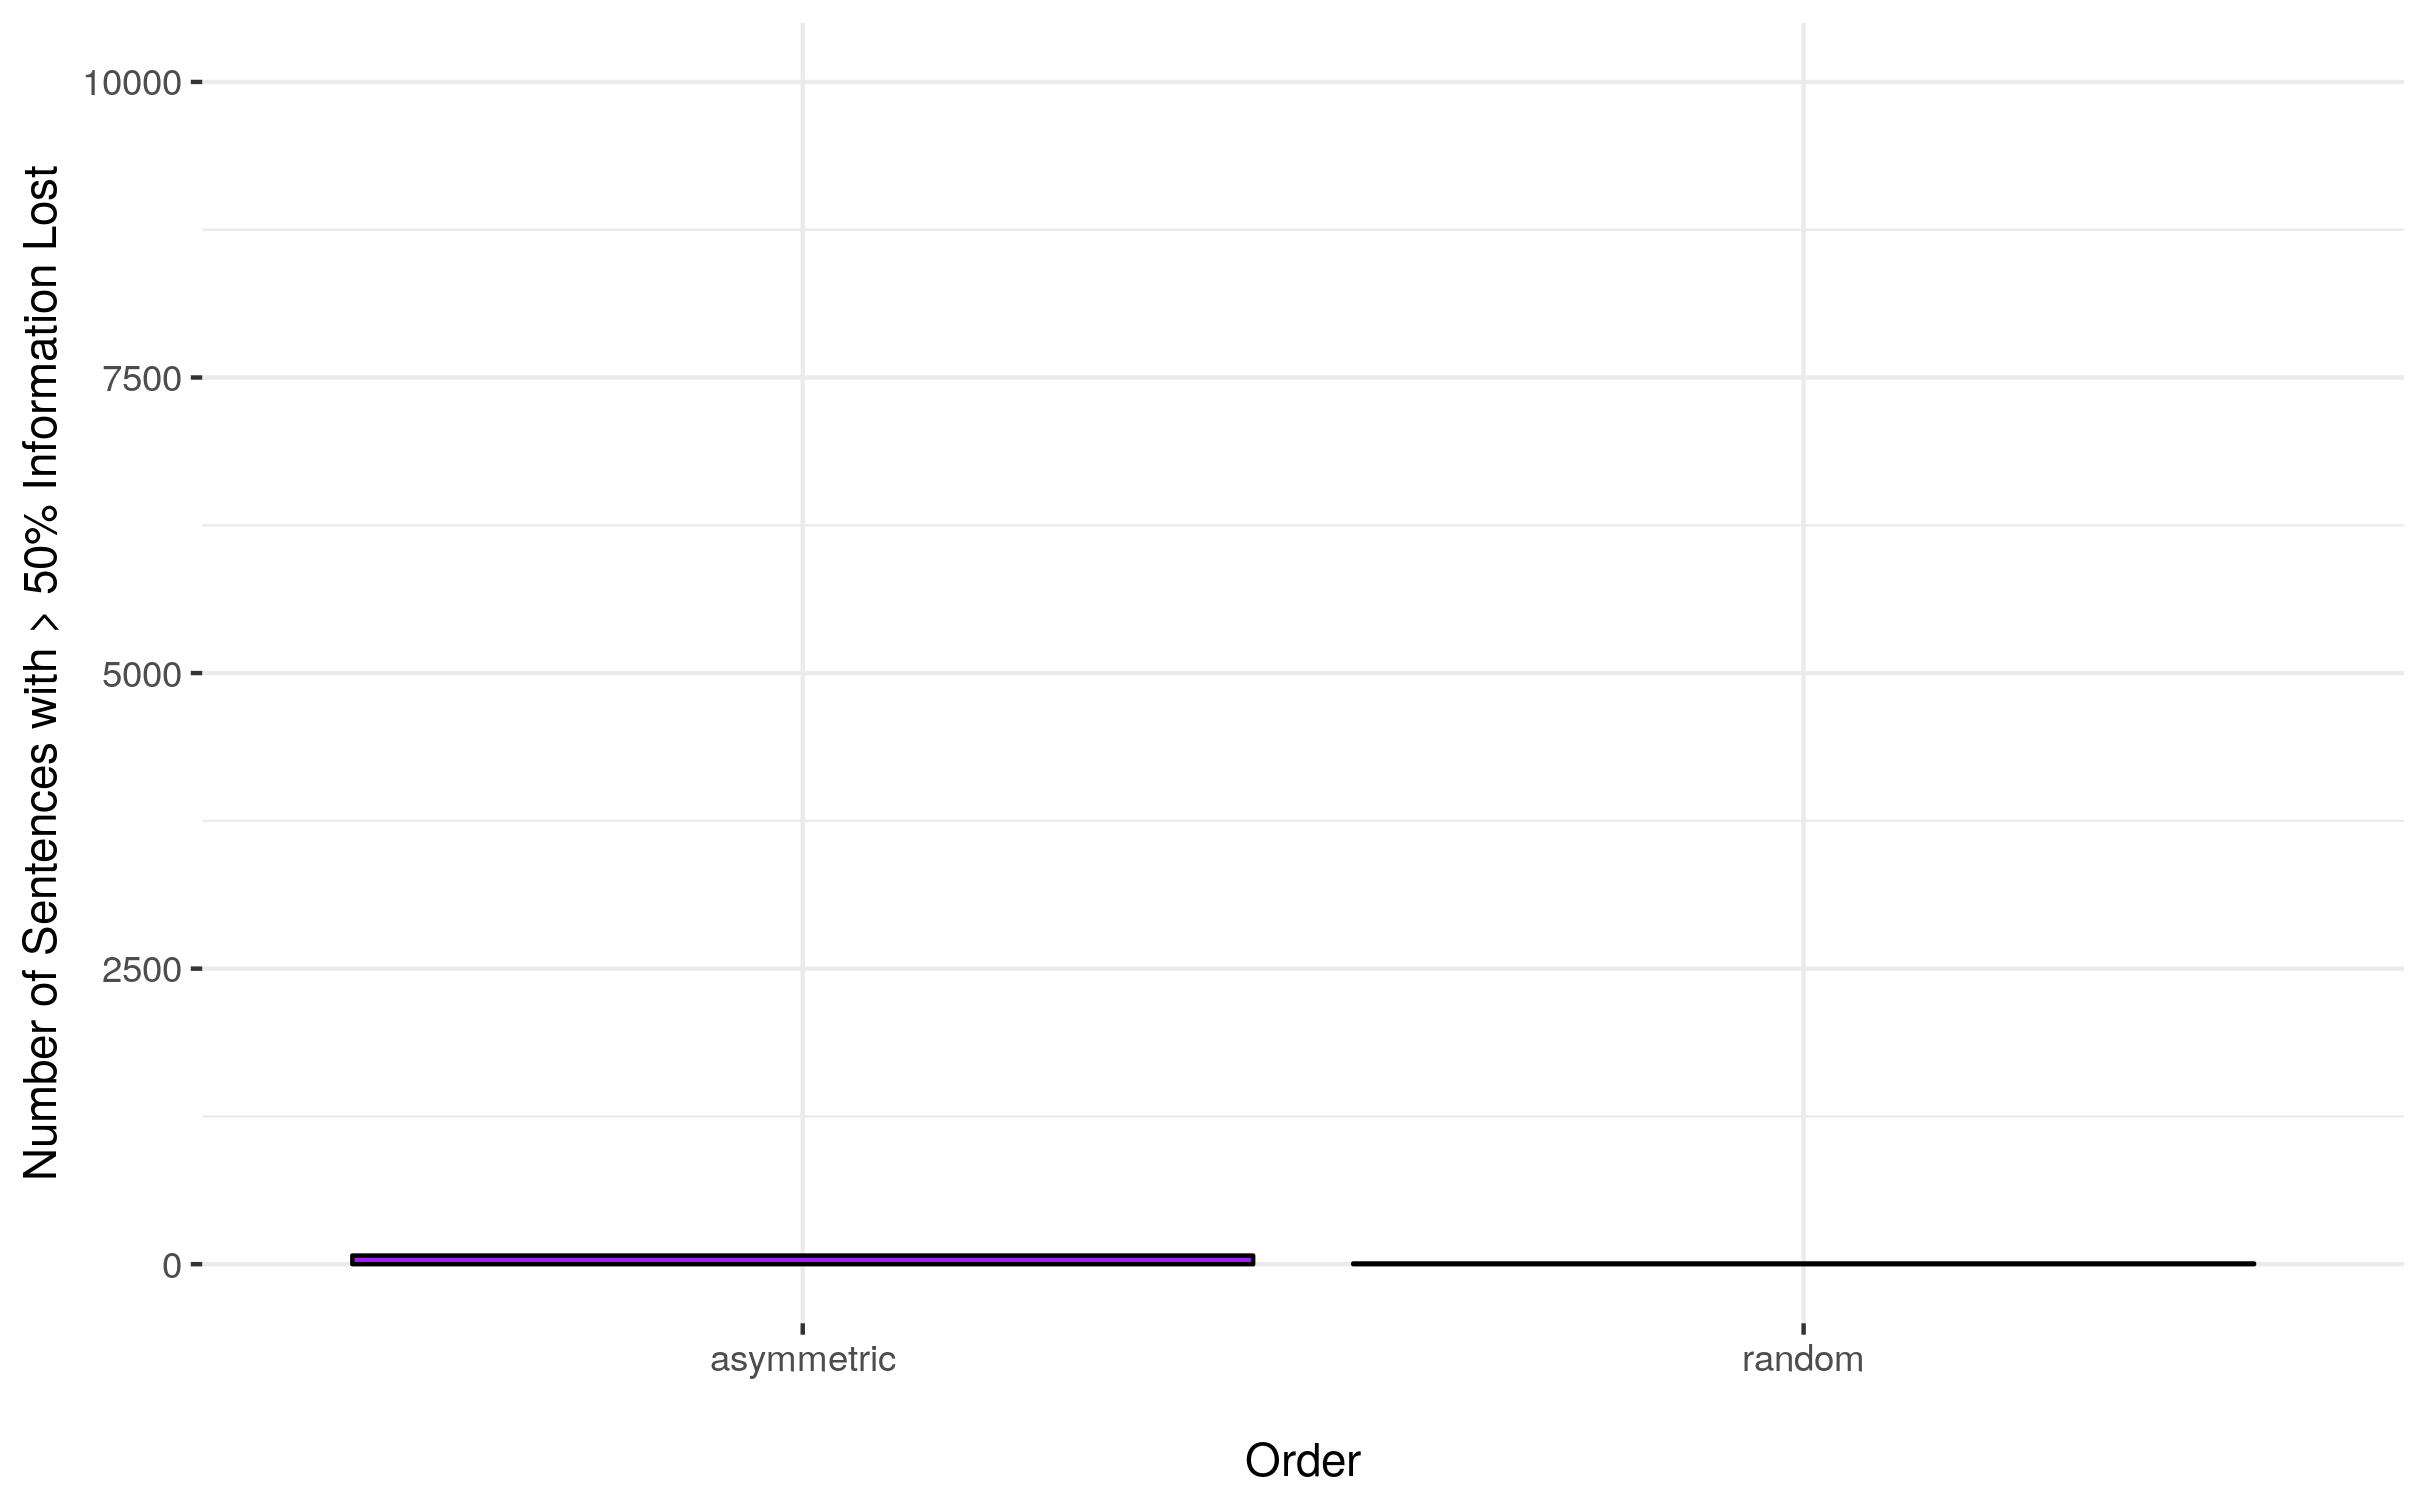
\includegraphics[width=1.115\textwidth]{uid-sim-majority.png}
\caption{>50\% information loss in 10,000 pseudo-sentences. (Loess curves on binary data.)}
\label{sim}
\end{center}
\end{figure}

Figure \ref{sim} shows that the UIDO-version of the strings resulted in the fewest catastrophic communication failures, even though those orders do not perform better than the asymmetric order in terms of overall proportion of bits lost across all the sentences. This means that, on average, the UIDO and asymmetric orders lose roughly the same amount of information per sentence (calculated as a proportion of the total amount of information in each sentence, so we can compare across sentences). However, the UIDO order is more likely to lose small or moderate amounts, while the asymmetric order is more likely to lose catastrophic amounts in some cases and small amounts in others. The randomized order fared worse than either the UIDO or asymmetric orders on the proportion of bits lost, and on the number of sentences lost to catastrophic communication failure, the randomized order fared better than the asymmetric order but worse than the UIDO order. The randomized order is clearly less adaptive for communication than the UIDO order on both measures, though the asymmetric order is the clear loser in preventing catastrophic communication failures.

Our simulation showed that the most uniform and least clumpy order (UIDO) is the most adaptive order for facilitating communication in a noisy channel, if the most important thing is to prevent the catastrophic loss of most of the information in an utterance. If the goal is simply to maximize transmission of all information overall, then the UIDO order performs better than the randomized order, and no worse that the clumpiest, asymmetric order. Therefore, there may well be a communicative advantage to uniformity, independent of the length of the signal (or amount of redundancy, which is equivalent in information theoretic terms). But even more strongly, if linguistic communication is mostly concerned with transmitting the message behind each utterance and avoiding catastrophic losses of that message, such that the information content groups in sub-parts of different utterances are not readily comparable to each other, then the results above show uniform orders to be much more adaptive for linguistic communication in noise. The intuition is: from the hearer's point of view, it's worse to lose any whole utterance or speech act than it is to lose 25\% of a few of them.


\section{Why? Duality (and more-ity) of patterning}
\label{moreity}

Now that it's clear uniformity does not uniquely protect against all information loss due to noise, per se, but rather to catastrophic information loss at the utterance level, do we have any \textsl{a priori} reason to think catastrophic information loss in an utterance is more dire than overall amount of information lost across utterances? 

The answer is yes, because %duality of patterning

Propositional content is, to some extent, a property of entire utterances (or clauses, at least), and it is definitely always a product of predicate-argument relations holding between constituents above the phoneme, morpheme, and word levels. Because that is the case, and it is the propositional content (and/or overall social function) of the utterance that the speaker will be primarily trying to reconstruct, it is possible that perceiving 70\% of an utterance's word-level information content will be sufficient for reconstructing 100\% of the propositional information or social function of the utterance. However, the fact that the words/morphemes map only larger meaningful linguistic units also means that hearing 30\% of the word-level information content may well not be enough to reconstruct the proposition. And if the hearer is unlucky enough that the noise destroyed some entire argument-predicate relations, then 30\% of the word-level information content may well mean the hearer has access to less than 30\% of event-level information the speaker intended to signal in the utterance, and possibly none of social/pragmatic function of the utterance (e.g. if it was primarily intended to signal desire to end an interaction, which must be inferred from the relevance of the entire proposition to the discourse). 

%Stated in terms of the information theoretic notion of \textsl{mutual information}, i.e. the there is probably a threshold of word-level mutual information below which it has knock on effects on the mutual information at the phrasal or higher levels such that this is not proportionately less than the word-level mutual information, but a lot less. The function of noise-resistant coding strategies, of which information uniformity could be one, is to keep the mutual information as high as possible for any level of noise. But in this case, uniformity itself doesn't increase mutual information, which is an average amount of information over signal transmissins, but rather, it tightens the variance of how much information is lost in any individual signal transmission such that lost information doesn't reach above the critical threshold as often as it might.

%For example, if noise disrupts the beginning of (\ref{relex}b), there's a big difference for reconstructing the speaker's intended proposition between having 30\% of the phonological words and 50\%: ``who's very important'' vs. ``that room who's very important''. 
 
Since language evolved in the context of an organism with remarkable capacities for categorical perception and inference, it is not surprising that linguistic structure at a given level must be inferred from some imperfect signal from linguistic structure at another level, provided enough of the signal is detected through the noise to make the inference. This isn't then just an issue for propositions, events, or predicate argument relations, but potentially an issue at every level of linguistic structure. We could conceive of linguistic comprehension as a daisy-chain of signaling, where the message for one signal becomes the signal for the next level of structure up. Take, for example, the following classic example of syntactic ambiguity:

\begin{exe}
	\ex I saw the astronomer with a telescope.
\end{exe}

\noindent For a hearer, the acoustics of \textsl{astronomer} serve as a signal for the message of phonological segments (including allophones), which the hearer perceives as categories drawn from a set of possible segments in their language. The segments, which were a message, now serve as a signal for the phonemes in \textsl{astronomer} and its syllabic parse, helping the hearer narrow down the relevant phonemes from their language's phonemic inventory and relevant parse from possible parses. The phonemes and syllables, the previous message, now serve as signals for the phonological word \textsl{astronomer}. The word, previously the message, is now the signal for two kinds of messages: its lexical meaning, selected from possible lexical meanings in the hearer's head, and the syntactic parse. Because of course, this sentence famously contains a PP-attachment ambiguity: the PP \textsl{with a telescope} could attach high, modifying the \textsc{see}ing event, or low, modifying \textsl{astronomer}. Such a PP probably attaches high more often than not in general (i.e. that outcome has a higher \textsl{source} probability), but \textsl{astronomer} serves as a signal to the hearer for the low attachment that ultimately means the astronomer has the telescope. The syntactic parse then constrains the set of possible higher meanings.

The signaling does not necessarily have to take place in the order I've indicated, and different directions of signaling probably happen at the same time. The point is, each inferred piece of linguistic structure at a given level, chosen probabilistically from a set of possible structures with help from the previous signal, can then in turn serve as a signal for yet another level of structure. In fact, it could be that the mechanism of inference is actually the human ability to generate appropriate sets of possible messages (i.e. structures) at multiple linguistic and pragmatic levels simultaneously, including the level of social function of an entire utterance. 
 %Or maybe: there is such a threshold effect at every linguistic level, so that meaning is recoverable...but then shouldn't it be a general property of all information? Maybe it is, at least for all information where the code is representing some larger categorical level, acoustics to segment (incl allophones), segment to phoneme, phoneme to morpheme, etc. ...so it won't be true for e.g. digital images, because however many pixels you have left you still have...but from the perspective of the human trying to decipher the picture. 

\section{Conclusion}

These methods are fast enough to be easily implementable in a variety of computational applications, and they provide insight into exactly how information uniformity guards against noise in language.

Beyond simulation, these methods allow for the rapid assessment informational uniformity of a variety of large natural language corpora during my fellowship, especially those with multi-person discourses.

\section*{Supplementary files}

\section*{Acknowledgments}

Thanks, Tom, for ``clumpy''. Thanks Tony.

\section*{Competing interests}

The authors have no competing interests to declare.


\bibliographystyle{linquiry2}
\bibliography{joelrefs}

\end{document}
